\documentclass[nobib]{tufte-handout}

%\\geometry{showframe}% for debugging purposes -- displays the margins

\newcommand{\bra}[1]{\left(#1\right)}
\usepackage{amssymb}
\usepackage{hyperref}
\usepackage{pgfplots}
\usepackage[activate={true,nocompatibility},final,tracking=true,kerning=true,spacing=true,factor=1100,stretch=10,shrink=10]{microtype}
\usepackage{color}
\usepackage{steinmetz}
% Fixes captions and images being cut off
\usepackage{marginfix}
\usepackage{array}
\usepackage{tikz}
\usepackage{amsmath,amsthm}
\usetikzlibrary{shapes}
\usetikzlibrary{positioning}
\usepackage{listings}
\usepackage{caption}
\DeclareCaptionFont{white}{\color{white}}
\DeclareCaptionFormat{listing}{\colorbox{gray}{\parbox{\textwidth}{#1#2#3}}}
\captionsetup[lstlisting]{format=listing,labelfont=white,textfont=white}

% Set up the images/graphics package
\usepackage{graphicx}
\setkeys{Gin}{width=\linewidth, totalheight=\textheight, keepaspectratio}
\graphicspath{{.}}

\title{Notes for ECON 25100 - Microeconomics}
\author[Shubham Saluja Kumar Agarwal]{Shubham Saluja Kumar Agarwal}
\date{\today}  % if the \date{} command is left out, the current date will be used

% The following package makes prettier tables.  We're all about the bling!
\usepackage{booktabs}

% The units package provides nice, non-stacked fractions and better spacing
% for units.
\usepackage{units}

% The fancyvrb package lets us customize the formatting of verbatim
% environments.  We use a slightly smaller font.
\usepackage{fancyvrb}
\fvset{fontsize=\normalsize}

% Small sections of multiple columns
\usepackage{multicol}

% For finite state machines 
\usetikzlibrary{automata} % Import library for drawing automata
\usetikzlibrary{positioning} % ...positioning nodes
\usetikzlibrary{arrows} % ...customizing arrows
\tikzset{node distance=2.5cm, % Minimum distance between two nodes. Change if necessary.
    every state/.style={ % Sets the properties for each state
    semithick,
    fill=gray!10},
    initial text={}, % No label on start arrow
    double distance=2pt, % Adjust appearance of accept states
    every edge/.style={ % Sets the properties for each transition
    draw,
    ->,>=stealth', % Makes edges directed with bold arrowheads
    auto,
    semithick}}
\let\epsilon\varepsilon

% These commands are used to pretty-print LaTeX commands
\newcommand{\doccmd}[1]{\texttt{\textbackslash#1}}% command name -- adds backslash automatically
\newcommand{\docopt}[1]{\ensuremath{\langle}\textrm{\textit{#1}}\ensuremath{\rangle}}% optional command argument
\newcommand{\docarg}[1]{\textrm{\textit{#1}}}% (required) command argument
\newenvironment{docspec}{\begin{quote}\noindent}{\end{quote}}% command specification environment
\newcommand{\docenv}[1]{\textsf{#1}}% environment name
\newcommand{\docpkg}[1]{\texttt{#1}}% package name
\newcommand{\doccls}[1]{\texttt{#1}}% document class name
\newcommand{\docclsopt}[1]{\texttt{#1}}% document class option name

% Define a custom command for definitions and biconditional
\newcommand{\defn}[2]{\noindent\textbf{#1}:\ #2}
\let\biconditional\leftrightarrow

\begin{document}

\maketitle

\begin{abstract}
    These are lecture notes for spring 2024 ECON 25100 at Purdue as taught by Professor Abigail Banan. Modify, use, and distribute as you please.
\end{abstract}

\tableofcontents

\section{Course Introduction}
This course offers a comprehensive exploration of the principles that govern
individual economic decision-making and the interactions within markets.

\pagebreak

\section{Introduction to Economic Principles}
\textit{This section will briefly define several important terms, topics,and principles relevant to the rest of this class.}\\~\\
Economics is the study of allocation of scarce resources to meet the unlimited
human wants.
\begin{itemize}
    \item Microeconomics: decision-making by individual economic agents such as firms and
          consumers.
    \item Macroeconomics: aggregate performance of the entire economic system.
    \item Empirical economics: facts to present a description of economic activity.
    \item Economic theory: relies upon principles to analyze behavior of economic agents.
\end{itemize}
Economy has slowly transitioned from mainly theoretical to mainly empirical.\\
Assumptions are made consistently, to more rigurously create a methodology to analyze the world without overly complicating things.\\
Model building is the creation of abstractions from reality.\\
\quad Occam's razor: The best model is that which describes reality and is the simplest.\\
\quad "Ceteris Paribus": All other things equal. (changing only certain parameters and leaving everything else the same)\\
\quad The lack of assumptions would make things either to simple or too complicated to viably describe reality.\\
\quad Economics provides a method to make a rational choice.\\
\quad Rigurous models are made to predict human behavior through either inductive logic, or deductive logic.\\
There are two kinds of economics:
\begin{itemize}
    \item Positive Economics: concerned with reality.
    \item Normative economics: concerned with what should be. (If a statement has
          "should" it's probably normative).
\end{itemize}
\quad The economic problem involves the allocation or resources among comepting wants.\\
\quad This exists due to scarcity.\\
\quad Scarcity exists because of unlimited human wants and limited resources.\\~\\
Economic Resources:\\
\begin{itemize}
    \item Land - space, natural resources.
    \item Capital - physical assets like factories or tractors.
    \item Labor - skills, abilities, knowledge, etc.
    \item Entrepeneurial talent - the economic agent who creates the enterprise.
    \item Technology - a manner in which resources are combined to produce commodities
          (methods of making processes more efficient).
\end{itemize}
Core Principles of Economics:
\begin{itemize}
    \item Cost-Benefit Principle: cost and benefits are the incentives. Do something if
          the benefits outweigh the costs. (Convert everything to money, and then
          calculate).\\ The cost-benefit principle is directly related to the willingness
          to pay, which is precisely, the conversion of benefits to money.\\ If the
          benefit is greater than the cost, one has achieved an economic surplus. This
          principle aims to maximize the economic surplus.\\ It also relates to framing
          effects, which is when a decision is affected by the method in which the
          situation or object is framed.
    \item Opportunity Cost Principle: The allocation of resources implies decisions and
          choices. For every choice we make, there are other choices we do not, and the
          next best alternative has a cost, which is known as the opportunity cost. \\
          This principle focuses on the trade-offs of particular options.\\ The
          opportunity cost is not the sum of all lost options, only the next best one.\\
          All choices involve trade-offs due to scarcity. The usage of resources on one
          choice limits the amount available for other choices.\\ \textit{Note: a sunk
              cost is a cost that cannot be recouped, and should be ignored. They should not
              be included into the current decision.}\\ As a subtopic of Opportunity Cost
          Principle is the Production Possibilities Frontier, which analyzes the
          different set of attainable gains based on different allocations. Under the
          assumption that the costs and benefits are constant, the graph will look
          something like this:
          \begin{center}
              \begin{tikzpicture}[scale = 0.7]
                  \begin{axis}[
                          axis lines = left,
                          xlabel = Choice 1,
                          ylabel = Choice 2,
                          ymax = 20,
                          xmax = 6,
                      ]
                      \addplot [
                          domain=0:5,
                          samples=100,
                          color=red,
                      ]
                      {-3*x + 15};
                  \end{axis}
              \end{tikzpicture}
          \end{center}
          Any allocation of time below the PPF is an inefficient use of resources.\\ Points above it are unreachable unless new productivity increase methods are found.\\
    \item Marginal Principle: Decisions about quantities are best made incrementally.
          Instead of analyzing how many, one should analyze whether smaller increases are
          viable and reasonable.\\ \quad Marginal Benefit: Benefit on an extra unit.\\
          \quad Marginal Cost: Cost of an extra unit.\\ While the marginal benefit of an
          additional unit exceeds it costs, it should be acquired.\\ Anything that asks
          how many can be analyzed marginally.\\ Economic surplus is maximized when the
          marginal cost equals the marginal benefit.
    \item Interdependence Principle: Your best choice depend on your other choices, the
          choices others make, development of markets, expectations of the future. When
          these factors change, the best choice might change as well. \\\quad Because you
          have limited resources, all the choices you make, affect others. \\\quad The
          choices made by other economic actors shape the choices available to you.
          \\\quad Changes in price and opportunities in one market affect your ability to
          make choices in others.\\\quad There is also a dependence through time, as
          choices you make now will have an effect on what you can do in the future.\\
\end{itemize}
\section{Demand \& Supply}
\subsection{Demand}
A demand curve is a function that shows the quantity demanded at different
price.\\ Quantity demanded is what buyers want to buy and are able to buy at
the given price.\\ Demand refers to the entire curve, while quantity demanded
is a point on the curve.\\
\begin{center}
    \begin{tikzpicture}[scale = 0.7]
        \begin{axis}[
                axis lines = left,
                xlabel = Quantity,
                ylabel = Price,
                ymax = 40,
                xmax = 6,
                ymin = 0,
                xmin = 0,
                legend entries = {demand}
            ]
            \addplot [
                domain=1:5,
                samples=10,
                color=red,
            ]
            {-7*x + 38};
        \end{axis}
    \end{tikzpicture}
\end{center}
The Demand Schedule and Curve are the tabular and graphical representations of the supply and demand curve.\\
The Law of Demand states that a demand curve will have a negative slope.\\
Utility: the happiness from the consumption of goods.\\
Marginal Utility: the change in utility derived from the consumption of one more unit of the good.\\
The demand curves show the marginal benefit. Thus, the demand curve is also the marginal benefits curve.\\
Diminishing Marginal Utility: the utility derived from consuming one more good is less than the one before. This ends up in a lower willingness to pay for the additional unit.\\
IMPORTANT: Keep buying until \textbf{price = marginal benefit}.\\
A demand function is typically written as $Q_d=f(P)$, but we prefer to plot the inverse demand function $P = f^{-1}(Q_d)$.\\
The Market Demand shows the aggregate of all individual demand curves, which we were discussing prior to this.
The change in price causes movement along the demand curve, as the change is endogenous (from inside the system).\\
So, if the price increases, the quantity demanded will decrease.\\
However, the exogenous changes, caused the curve to shift:
\begin{itemize}
    \item Population
    \item Expectations
    \item Seasons
    \item Tastes (fashion)
    \item Income:
          \begin{itemize}
              \item Normal Goods: good for which demand increases alongside increase of income.
              \item Inferior Goods: good for which demand decreases with income increases.
          \end{itemize}
    \item Prices of related goods:
          \begin{itemize}
              \item Substitutes-in-consumption: if two things can be replaced, the decrease in the
                    price leads to the increase of the other.
              \item Complements-in-consumption: it two things are used together, the increase in
                    the price of one leads to a decrease in the demand of the other.
          \end{itemize}
\end{itemize}
When external factors change, that is, not the price, the demand shifts as well.
\begin{center}
    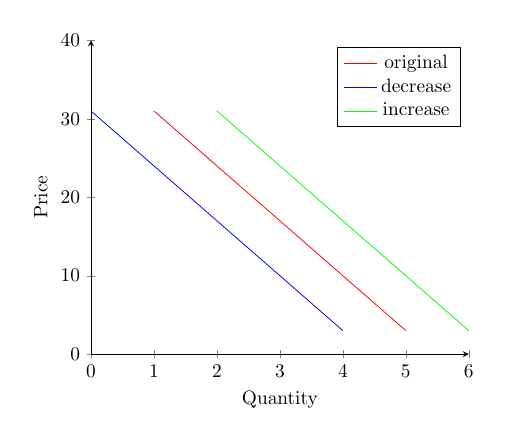
\begin{tikzpicture}[scale = 0.7]
        \begin{axis}[
                axis lines = left,
                xlabel = Quantity,
                ylabel = Price,
                ymax = 40,
                xmax = 6,
                ymin = 0,
                xmin = 0,
                legend entries = {original, decrease, increase}
            ]
            \addplot [
                domain=1:5,
                samples=10,
                color=red,
            ]
            {-7*x + 38};
            \addplot [
                domain=0:4,
                samples=10,
                color=blue,
            ]
            {-7*x + 31};
            \addplot [
                domain=2:6,
                samples=10,
                color=green,
            ]
            {-7*x + 45};
        \end{axis}
    \end{tikzpicture}
\end{center}
So, price changes quantity demanded, everything else shifts the demand, either positively or negatively.
\subsection{Supply}
The supply curve is a function that shows the quantity supplied at different
prices. Quantity supplied is the amount that suppliers are willing and able to
supply at a price. \\ NOTE: supply is the curve, quantity supplied is a
point.\\
\begin{center}
    \begin{tikzpicture}[scale = 0.7]
        \begin{axis}[
                axis lines = left,
                xlabel = Quantity,
                ylabel = Price,
                ymax = 40,
                xmax = 6,
                ymin = 0,
                xmin = 0,
                legend entries = {supply}
            ]
            \addplot [
                domain=1:5,
                samples=10,
                color=blue,
            ]
            {6*x + 2};
        \end{axis}
    \end{tikzpicture}
\end{center}
The supply curve, unlike the demand curve has a positive slope.\\
More price means more supply.\\
The marginal cost for selling one more unit is the focus of this curve.\\
The opportunity cost from producing the additional good minus the additional production costs.\\
Variable costs are costs that vary with quantity, while fixed remain constant.\\
NOTE: the supply curve is also your marginal cost curve.\\
Marginal product is the increase in output from an additional labor unit.\\
It diminishes with each additional labor unit. It can occur when some of your inputs are fixed.\\
Marginal costs of production rise, which causes the positive slope of the supply curve.\\
More input costs lead to rising marginal costs, as the production requirements increase.\\
The marginal benefit is the gain from the additional unit.\\
As price increases, producers will be more willing to produce more.\\
Once again, continue producing until $\mathbf{MC=MB}$, or until price and marginal costs are equal.\\
The supply function is $Q_s=f(P)$, but the plot is the inverse, $P=f^{-1}(Q)$.\\
Individual Supply shows a firm's willingness to produce and sell at different prices. Market supply is the sum of all individual price curves.\\
The market one is in influences the decisions made. The supply depends on the market price. This class will start by analyzing a perfectly competitive market, in which everyone sells the exact same product, and there are many suppliers and buyers.\\
This does not usually exist in real life, which would cause sellers to not be price-takers.\\
A change in price causes movement along the supply curve, changing quantity supplied.\\
Supply curves are shifted by
\begin{itemize}
    \item Input Prices
    \item Productivity and Technology
    \item Prices of related items:
          \begin{itemize}
              \item Substitutes-in-production: Alternate use of resources, goods that can be made
                    with the same resources.
              \item Complements-in-production: Goods made together, like byproducts, or scrap
                    usage.
          \end{itemize}
    \item Expectation of the future
    \item Type and number of sellers
\end{itemize}
A supply shift looks like the following:
\begin{center}
    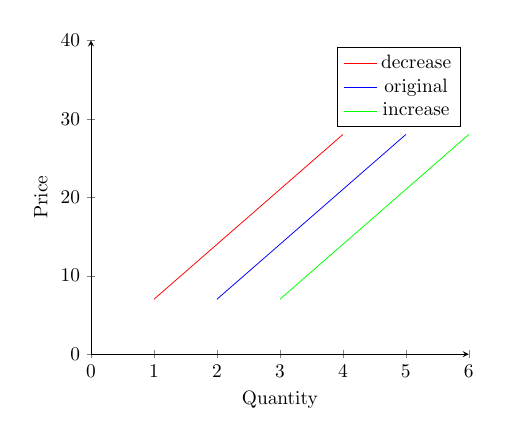
\begin{tikzpicture}[scale = 0.7]
        \begin{axis}[
                axis lines = left,
                xlabel = Quantity,
                ylabel = Price,
                ymax = 40,
                xmax = 6,
                ymin = 0,
                xmin = 0,
                legend entries = {decrease, original, increase}
            ]
            \addplot [
                domain=1:4,
                samples=10,
                color=red,
            ]
            {7*x };
            \addplot [
                domain=2:5,
                samples=10,
                color=blue,
            ]
            {7*x - 7};
            \addplot [
                domain=3:6,
                samples=10,
                color=green,
            ]
            {7*x - 14};
        \end{axis}
    \end{tikzpicture}
\end{center}
\section{Markets and Equilibrium}
Markets are organized by what is produced, who produces it, how they are
produced, and who gets the product. There are two kinds of economies:
\begin{itemize}
    \item Planned economies: These decisions are made by a central power
    \item Market economies: Each person makes their own decisions
\end{itemize}
A market is what connects buyer and sellers through goods or services.\\
They can be places or websites. There are several types, such as monopolies, oligopolies, etc.\\
Equilibrium is the point at which the market ceases to change. It is when quantity supplied and quantity demanded are equal,
This defines equilibrium quantity as the quantity demanded in equilibrium and the equilibrium price as the price of a product at equilibrium.\\
Every seller finds a buyer, and every buyer finds a seller. The balance created by this allows there to be no changes.\\
There is no shortage or surplus, which are Q. demanded> Q. supplied and the opposite respectively.\\
This looks like the following when represented graphically:
\begin{center}
    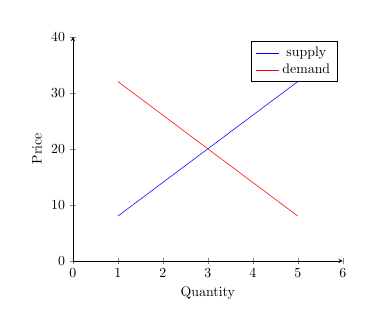
\begin{tikzpicture}[scale = 0.5]
        \begin{axis}[
                axis lines = left,
                xlabel = Quantity,
                ylabel = Price,
                ymax = 40,
                xmax = 6,
                ymin = 0,
                xmin = 0,
                legend entries = {supply, demand}
            ]
            \addplot [
                domain=1:5,
                samples=10,
                color=blue,
            ]
            {6*x + 2};
            \addplot [
                domain=1:5,
                samples=10,
                color=red,
            ]
            {-6*x + 38};
        \end{axis}
    \end{tikzpicture}
\end{center}

The system of equations to solve is:
\begin{align*}
    Q_d & = -a_1P+c_1 \\
    Q_s & = a_2P-c_2  \\
    Q_s & =Q_d
\end{align*}
Where the searched for, and relevant variables are $P$ and $Q$ (not $Q_s$ and $Q_d$ separately, as they are equal).\\
If the market is not in equilibrium, that is, it is in disequilibrium, which are marked by:
\begin{itemize}
    \item Queuing: People trying to get stuff and not succeeding.
    \item Bundling of extras: promotions, 2 for 1, etc.
    \item Secondary Markets: people buying and reselling.
\end{itemize}
If market price > equilibrium price, surplus will occur, and thus market forces will force the price to reach equilibrium.
Surplus is $Q_s(P_H)-Q_d(P_H)$ with $P_H$ being the high price.
\begin{center}
    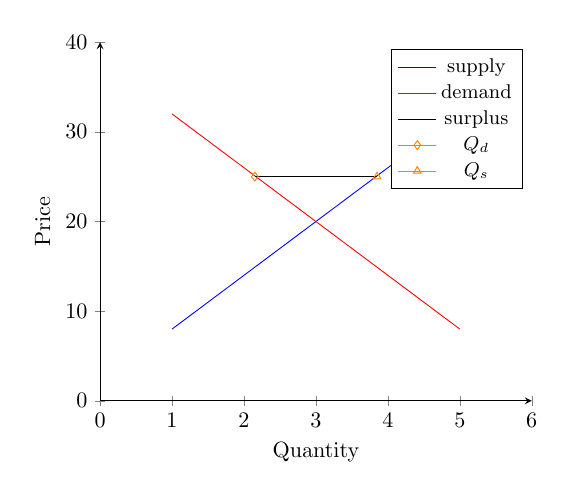
\begin{tikzpicture}[scale = 0.8]
        \begin{axis}[
                axis lines = left,
                xlabel = Quantity,
                ylabel = Price,
                ymax = 40,
                xmax = 6,
                ymin = 0,
                xmin = 0,
                legend entries = {supply, demand, surplus, $Q_d$, $Q_s$},
                legend style = {font=\small}
            ]
            \addplot [
                domain=1:5,
                samples=10,
                color=blue,
            ]
            {6*x + 2};
            \addplot [
                domain=1:5,
                samples=10,
                color=red,
            ]
            {-6*x + 38};
            \addplot [
                domain=2.15:3.85,
                samples=10,
                color=black,
            ]
            {0*x+25};
            \addplot [orange, mark=diamond] coordinates {(2.15,25)};
            \addplot [orange, mark=triangle] coordinates {(3.85,25)};
        \end{axis}
    \end{tikzpicture}
\end{center}
The shortage in a market is calculated by $Q_d-Q_s$ at a low price $P_L$.
Which looks like this:
\begin{center}
    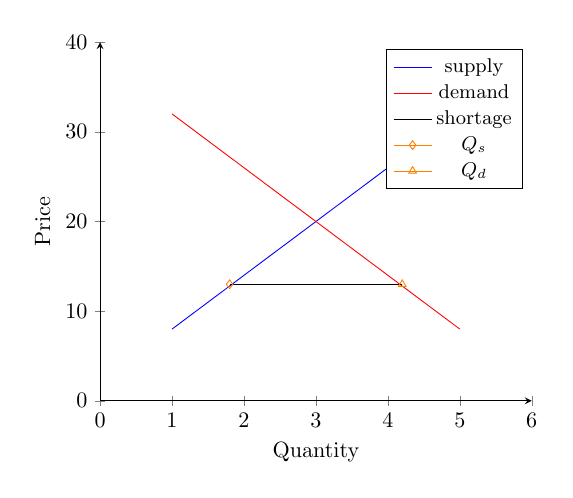
\begin{tikzpicture}[scale = 0.8]
        \begin{axis}[
                axis lines = left,
                xlabel = Quantity,
                ylabel = Price,
                ymax = 40,
                xmax = 6,
                ymin = 0,
                xmin = 0,
                legend entries = {supply, demand, shortage, $Q_s$, $Q_d$},
                legend style = {font=\small}
            ]
            \addplot [
                domain=1:5,
                samples=10,
                color=blue,
            ]
            {6*x + 2};
            \addplot [
                domain=1:5,
                samples=10,
                color=red,
            ]
            {-6*x + 38};
            \addplot [
                domain=1.8:4.2,
                samples=10,
                color=black,
            ]
            {0*x+13};
            \addplot [orange, mark=diamond] coordinates {(1.8,13)};
            \addplot [orange, mark=triangle] coordinates {(4.2,13)};
        \end{axis}
    \end{tikzpicture}
\end{center}
\subsection{New Equilibrium}
Equilibrium can vary with:
\begin{itemize}
    \item Shifts in demand: if one of the demand shifters occurs, the demand curve will
          shift. This will cause the equilibrium to shift as well.
          \begin{itemize}
              \item Decrease in demand: decrease in equilibrium price and a decrease in equilibrium
                    quantity.
                    \begin{center}
                        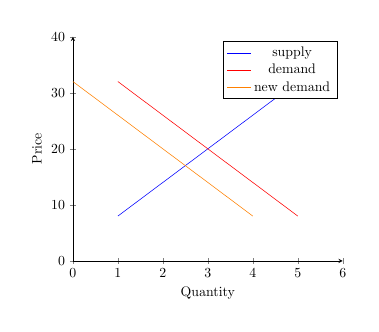
\begin{tikzpicture}[scale = 0.5]
                            \begin{axis}[
                                    axis lines = left,
                                    xlabel = Quantity,
                                    ylabel = Price,
                                    ymax = 40,
                                    xmax = 6,
                                    ymin = 0,
                                    xmin = 0,
                                    legend entries = {supply, demand, new demand}
                                ]
                                \addplot [
                                    domain=1:5,
                                    samples=10,
                                    color=blue,
                                ]
                                {6*x + 2};
                                \addplot [
                                    domain=1:5,
                                    samples=10,
                                    color=red,
                                ]
                                {-6*x + 38};
                                \addplot [
                                    domain=0:4,
                                    samples=10,
                                    color=orange,
                                ]
                                {-6*x + 32};
                            \end{axis}
                        \end{tikzpicture}
                    \end{center}
              \item Increase in demand: increase in equilibrium price and quantity.
                    \begin{center}
                        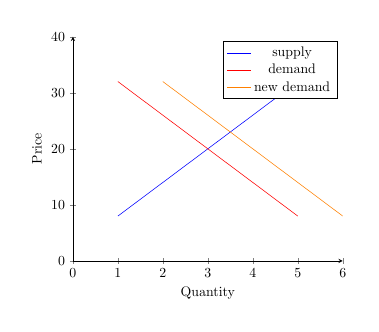
\begin{tikzpicture}[scale = 0.5]
                            \begin{axis}[
                                    axis lines = left,
                                    xlabel = Quantity,
                                    ylabel = Price,
                                    ymax = 40,
                                    xmax = 6,
                                    ymin = 0,
                                    xmin = 0,
                                    legend entries = {supply, demand, new demand}
                                ]
                                \addplot [
                                    domain=1:5,
                                    samples=10,
                                    color=blue,
                                ]
                                {6*x + 2};
                                \addplot [
                                    domain=1:5,
                                    samples=10,
                                    color=red,
                                ]
                                {-6*x + 38};
                                \addplot [
                                    domain=2:6,
                                    samples=10,
                                    color=orange,
                                ]
                                {-6*x + 44};
                            \end{axis}
                        \end{tikzpicture}
                    \end{center}
          \end{itemize}
    \item Shift in Supply: occurs when one of the supply shifters occurs. Once again, the
          market moves to a new equilibrium.
          \begin{itemize}
              \item Decrease in Supply: increase in equilibrium price and decrease in quantity.
                    \begin{center}
                        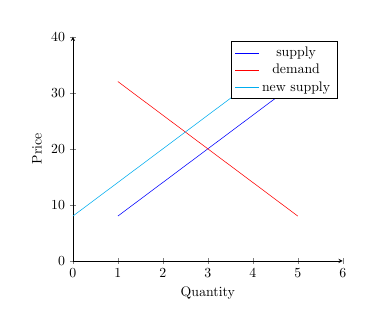
\begin{tikzpicture}[scale = 0.5]
                            \begin{axis}[
                                    axis lines = left,
                                    xlabel = Quantity,
                                    ylabel = Price,
                                    ymax = 40,
                                    xmax = 6,
                                    ymin = 0,
                                    xmin = 0,
                                    legend entries = {supply, demand, new supply}
                                ]
                                \addplot [
                                    domain=1:5,
                                    samples=10,
                                    color=blue,
                                ]
                                {6*x + 2};
                                \addplot [
                                    domain=1:5,
                                    samples=10,
                                    color=red,
                                ]
                                {-6*x + 38};
                                \addplot [
                                    domain=0:4,
                                    samples=10,
                                    color=cyan,
                                ]
                                {6*x + 8};
                            \end{axis}
                        \end{tikzpicture}
                    \end{center}
              \item Increase in Supply: decrease in equilibrium price and increase in quantity.
                    \begin{center}
                        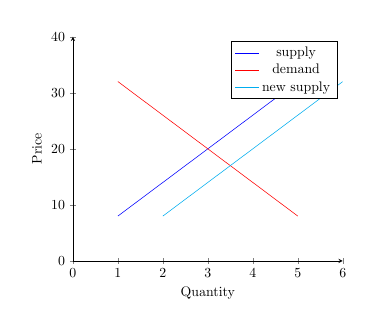
\begin{tikzpicture}[scale = 0.5]
                            \begin{axis}[
                                    axis lines = left,
                                    xlabel = Quantity,
                                    ylabel = Price,
                                    ymax = 40,
                                    xmax = 6,
                                    ymin = 0,
                                    xmin = 0,
                                    legend entries = {supply, demand, new supply}
                                ]
                                \addplot [
                                    domain=1:5,
                                    samples=10,
                                    color=blue,
                                ]
                                {6*x + 2};
                                \addplot [
                                    domain=1:5,
                                    samples=10,
                                    color=red,
                                ]
                                {-6*x + 38};
                                \addplot [
                                    domain=2:6,
                                    samples=10,
                                    color=cyan,
                                ]
                                {6*x -4};
                            \end{axis}
                        \end{tikzpicture}
                    \end{center}
          \end{itemize}
\end{itemize}
It is however, also possible for both demand and supply to shift. This may result in an ambiguous shift of equilibrium price and equilibrium quantity.\\
\begin{itemize}
    \item Demand $\uparrow$, Supply $\uparrow$ --- equilibrium price: (?), but
          equilibrium quantity: ($\uparrow$)
          \begin{center}
              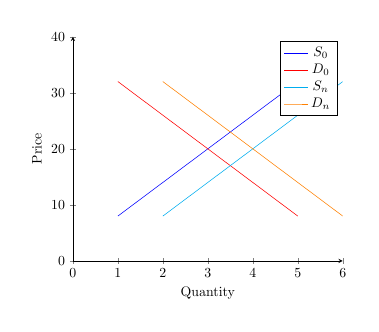
\begin{tikzpicture}[scale = 0.5]
                  \begin{axis}[
                          axis lines = left,
                          xlabel = Quantity,
                          ylabel = Price,
                          ymax = 40,
                          xmax = 6,
                          ymin = 0,
                          xmin = 0,
                          legend entries = {$S_0$, $D_0$, $S_n$, $D_n$}
                      ]
                      \addplot [
                          domain=1:5,
                          samples=10,
                          color=blue,
                      ]
                      {6*x + 2};
                      \addplot [
                          domain=1:5,
                          samples=10,
                          color=red,
                      ]
                      {-6*x + 38};
                      \addplot [
                          domain=2:6,
                          samples=10,
                          color=cyan,
                      ]
                      {6*x -4};
                      \addplot [
                          domain=2:6,
                          samples=10,
                          color=orange,
                      ]
                      {-6*x + 44};
                  \end{axis}
              \end{tikzpicture}
          \end{center}
    \item Demand $\downarrow$, Supply $\downarrow$ --- equilibrium price: (?), but
          equilibrium quantity: ($\downarrow$)
          \begin{center}
              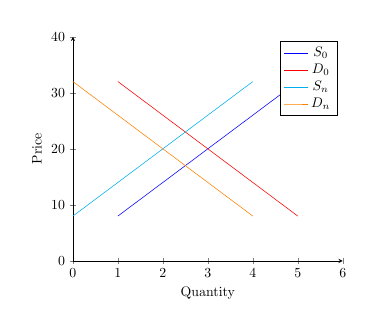
\begin{tikzpicture}[scale = 0.5]
                  \begin{axis}[
                          axis lines = left,
                          xlabel = Quantity,
                          ylabel = Price,
                          ymax = 40,
                          xmax = 6,
                          ymin = 0,
                          xmin = 0,
                          legend entries = {$S_0$, $D_0$, $S_n$, $D_n$}
                      ]
                      \addplot [
                          domain=1:5,
                          samples=10,
                          color=blue,
                      ]
                      {6*x + 2};
                      \addplot [
                          domain=1:5,
                          samples=10,
                          color=red,
                      ]
                      {-6*x + 38};
                      \addplot [
                          domain=0:4,
                          samples=10,
                          color=cyan,
                      ]
                      {6*x + 8};
                      \addplot [
                          domain=0:4,
                          samples=10,
                          color=orange,
                      ]
                      {-6*x + 32};
                  \end{axis}
              \end{tikzpicture}
          \end{center}
    \item Demand $\uparrow$, Supply $\downarrow$ --- equilibrium price: ($\uparrow$), but
          equilibrium quantity: (?)
          \begin{center}
              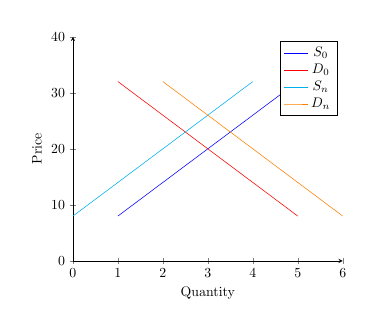
\begin{tikzpicture}[scale = 0.5]
                  \begin{axis}[
                          axis lines = left,
                          xlabel = Quantity,
                          ylabel = Price,
                          ymax = 40,
                          xmax = 6,
                          ymin = 0,
                          xmin = 0,
                          legend entries = {$S_0$, $D_0$, $S_n$, $D_n$}
                      ]
                      \addplot [
                          domain=1:5,
                          samples=10,
                          color=blue,
                      ]
                      {6*x + 2};
                      \addplot [
                          domain=1:5,
                          samples=10,
                          color=red,
                      ]
                      {-6*x + 38};
                      \addplot [
                          domain=0:4,
                          samples=10,
                          color=cyan,
                      ]
                      {6*x +8};
                      \addplot [
                          domain=2:6,
                          samples=10,
                          color=orange,
                      ]
                      {-6*x + 44};
                  \end{axis}
              \end{tikzpicture}
          \end{center}
    \item Demand $\downarrow$, Supply $\uparrow$ --- equilibrium price: ($\downarrow$),
          but equilibrium quantity: (?)
          \begin{center}
              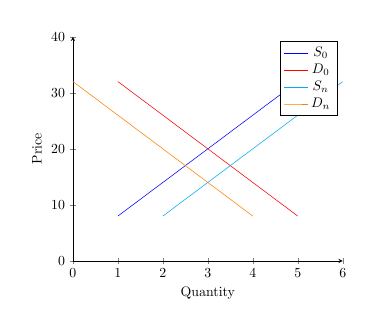
\begin{tikzpicture}[scale = 0.5]
                  \begin{axis}[
                          axis lines = left,
                          xlabel = Quantity,
                          ylabel = Price,
                          ymax = 40,
                          xmax = 6,
                          ymin = 0,
                          xmin = 0,
                          legend entries = {$S_0$, $D_0$, $S_n$, $D_n$}
                      ]
                      \addplot [
                          domain=1:5,
                          samples=10,
                          color=blue,
                      ]
                      {6*x + 2};
                      \addplot [
                          domain=1:5,
                          samples=10,
                          color=red,
                      ]
                      {-6*x + 38};
                      \addplot [
                          domain=2:6,
                          samples=10,
                          color=cyan,
                      ]
                      {6*x -4};
                      \addplot [
                          domain=0:4,
                          samples=10,
                          color=orange,
                      ]
                      {-6*x + 32};
                  \end{axis}
              \end{tikzpicture}
          \end{center}
\end{itemize}
Supply and demand can be used to predict and diagnose market outcomes.\\
All the previous analysis in this section leads to the following overall rules:
\begin{enumerate}
    \item If price and quantity move in same direction, demand has shifted, but we don't
          know what has happened to the supply.
    \item If price and quantity move in opposite directions, supply has shifted, but we
          don't know what has happened to the demand.
\end{enumerate}
\section{Elasticity}
Elasticity is a measure of the responsiveness to the changes in other
variables.
\begin{equation*}
    E_{x,y} = \frac{\%\Delta x}{\%\Delta y}
\end{equation*}
What is important about this are the sign and magnitude. It is positive if when $y$ increases, $x$ increases as well. The relationship is negative if when $y$ increases, $x$ decreases.\\
\begin{align*}
    |E_{x,y} & >1| \implies x \text{ is highly responsive to y, or the relationship is elastic} \\
    |E_{x,y} & <1| \implies x \text{ is slightly responsive to y, or inelastic}                 \\
    |E_{x,y} & =1| \implies x \text{ is proportionally responsive to y, or unitary elastic}
\end{align*}
\begin{itemize}
    \item Price elasticity of demand: A measure of how responsive buyers are to price
          changes.
          \begin{equation*}
              |\text{Price Elasticity of Demand}| = \frac{|\%\text{ change in quantity demanded}|}{|\%\text{ change in prices}|}
          \end{equation*}
          The negative value would mean nothing, as it is already predefined, and so, only the magnitude (or absolute value) is relevant.\\
          There are a few other methods:
          \begin{equation*}
              |E_D| = \left\vert \frac{100*\frac{Q_2-Q_1}{Q_1}}{100*\frac{P_2-P_1}{P_1}}\right\vert
          \end{equation*}
          which ignores direction, which is problematic, so you could use the midpoint formula method:
          \begin{equation*}
              |E_D| = \left\vert \frac{100*\frac{Q_2-Q_1}{(Q_2+Q_1)/2}}{100*\frac{P_2-P_1}{(P_2+P_1)/2}}\right\vert = \left\vert \frac{\frac{Q_2-Q_1}{(Q_2+Q_1)}}{\frac{P_2-P_1}{(P_2+P_1)}}\right\vert
          \end{equation*}
          Which is also referred to as "Arc Elasticity of Demand".\\~\\
          Perfectly Elastic demand has $E_D = \infty$. That is, you can change price as much as you want, and the demand will not change.\\
          Perfectly Inelastic demand has $E_D = 0$ which means the demand will shoot to 0 for any price change.\\
          An elastic curve would look like the following:
          \begin{center}
              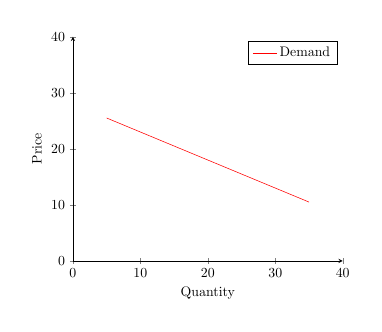
\begin{tikzpicture}[scale = 0.5]
                  \begin{axis}[
                          axis lines = left,
                          xlabel = Quantity,
                          ylabel = Price,
                          ymax = 40,
                          xmax = 40,
                          ymin = 0,
                          xmin = 0,
                          legend entries = {Demand}
                      ]
                      \addplot [
                          domain=5:35,
                          samples=10,
                          color=red,
                      ]
                      {-0.5*x + 28};
                  \end{axis}
              \end{tikzpicture}
          \end{center}
          While an inelastic curve would look more like the following:
          \begin{center}
              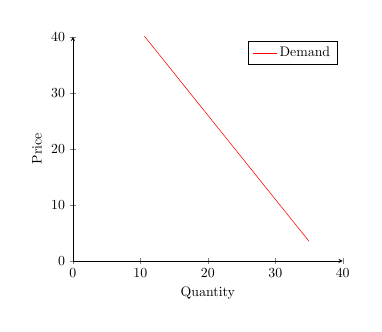
\begin{tikzpicture}[scale = 0.5]
                  \begin{axis}[
                          axis lines = left,
                          xlabel = Quantity,
                          ylabel = Price,
                          ymax = 40,
                          xmax = 40,
                          ymin = 0,
                          xmin = 0,
                          legend entries = {Demand}
                      ]
                      \addplot [
                          domain=5:35,
                          samples=10,
                          color=red,
                      ]
                      {-1.5*x + 56};
                  \end{axis}
              \end{tikzpicture}
          \end{center}
          Different factors, such as
          \begin{itemize}
              \item Availability of substitutes
              \item Duration of purchase horizon, that is how much time there is to purchase the
                    product
              \item Expenditure share of consumer budget, that is proportion of total income that
                    the purchase will consume
              \item Necessity or Luxury?
              \item Products with lower search costs, that is how easy it is to come across the
                    product
              \item Addiction
          \end{itemize}
          can affect the elasticity of demand.\\
          The elasticity varies along the demand curve. At a higher price, the elasticity is higher, as the formula indicates.
          \begin{center}
              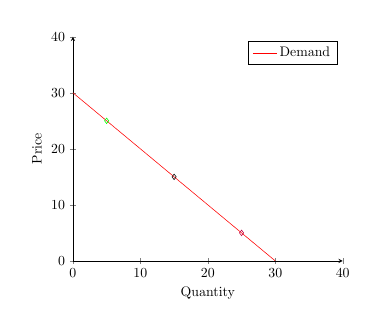
\begin{tikzpicture}[scale = 0.5]
                  \begin{axis}[
                          axis lines = left,
                          xlabel = Quantity,
                          ylabel = Price,
                          ymax = 40,
                          xmax = 40,
                          ymin = 0,
                          xmin = 0,
                          legend entries = {Demand}
                      ]
                      \addplot [
                          domain=0:30,
                          samples=10,
                          color=red,
                      ]
                      {-1*x + 30};
                      \addplot [black, mark=diamond] coordinates {(15,15)};
                      \addplot [green, mark=diamond] coordinates {(5,25)};
                      \addplot [purple, mark=diamond] coordinates {(25,5)};
                  \end{axis}
              \end{tikzpicture}
          \end{center}
          At the green diamond, if we were to use the midpoint formula, the elasticity would be quite high, while at the purple diamond, it would be low. The black diamond, which is the midpoint of the curve, would be unitary elastic.\\
          So, it would be unitary elastic at the point (Q, P) where $Q=\frac{y-intercept}{2}$ and $P = \frac{x-intercept}{2}$.\\
          Total revenue is defined as $P*Q$.\\ A change in price leads to a change in quantity demanded, in the opposite direction.\\
          The price of elasticity of demand tells us whether we should increase or decrease the price.\\
          One should decrease the price if the demand is elastic. One should increase the price if the demand is elastic. This allows us to draw the following plots:
          \begin{center}
              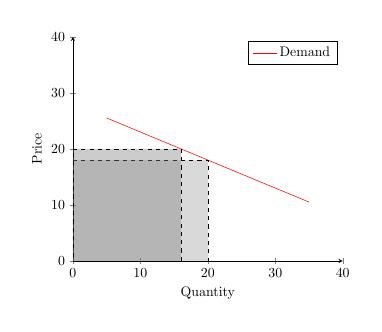
\begin{tikzpicture}[scale = 0.5]
                  \begin{axis}[
                          axis lines = left,
                          xlabel = Quantity,
                          ylabel = Price,
                          ymax = 40,
                          xmax = 40,
                          ymin = 0,
                          xmin = 0,
                          legend entries = {Demand}
                      ]
                      \addplot [
                          domain=5:35,
                          samples=10,
                          color=red,
                      ]
                      {-0.5*x + 28};
                      \addplot [black, dashed, fill=gray, fill opacity=0.3] coordinates {(0,18) (20,18) (20,0)} \closedcycle;
                      \addplot [black, dashed, fill=gray, fill opacity=0.4] coordinates {(0,20) (16,20) (16,0)} \closedcycle;
                  \end{axis}
              \end{tikzpicture}
              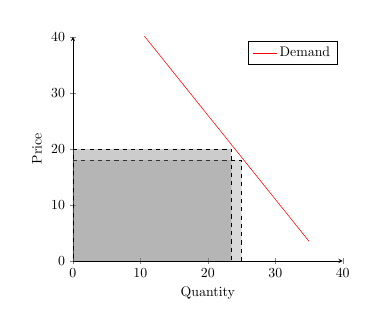
\begin{tikzpicture}[scale = 0.5]
                  \begin{axis}[
                          axis lines = left,
                          xlabel = Quantity,
                          ylabel = Price,
                          ymax = 40,
                          xmax = 40,
                          ymin = 0,
                          xmin = 0,
                          legend entries = {Demand}
                      ]
                      \addplot [
                          domain=5:35,
                          samples=10,
                          color=red,
                      ]
                      {-1.5*x + 56};
                      \addplot [black, dashed, fill=gray, fill opacity=0.3] coordinates {(0,18) (25,18) (25,0)} \closedcycle;
                      \addplot [black, dashed, fill=gray, fill opacity=0.4] coordinates {(0,20) (23.5,20) (23.5,0)} \closedcycle;
                  \end{axis}
              \end{tikzpicture}
          \end{center}
          It can be seen that an increase in price in the first graph would lead to a larger decrease in quantity, causing the revenue to fall. In the other one, we can see that an increase in price would only slightly decrease the quantity demanded, which is an increase in the revenue.\\
          Thus, we can conclude that the revenue also varies along the demand curve.\\
          The revenue looks like this:
          \begin{center}
              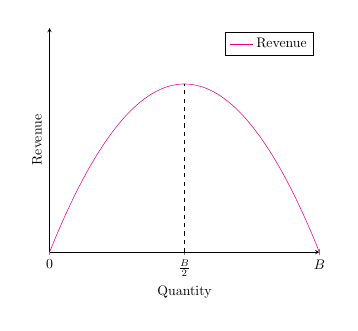
\begin{tikzpicture}[scale = 0.5]
                  \begin{axis}[
                          axis lines = left,
                          xlabel = Quantity,
                          ylabel = Revenue,
                          ymax = 40,
                          xmax = 40,
                          ymin = 0,
                          xmin = 0,
                          legend entries = {Revenue},
                          xtick={0, 20, 40},
                          xticklabels = {$0$, {$\frac{B}{2}$}, $B$},
                          ytick=\empty
                      ]
                      \addplot [
                          domain=0:40,
                          samples=100,
                          color=magenta,
                      ]
                      {-(0.075)*x^2 + 3*x};
                      \addplot [black, dashed] coordinates {(20,0) (20,30)};
                  \end{axis}
              \end{tikzpicture}
          \end{center}
          So, when the demand is unit elastic, the revenue is maximized.
    \item Cross-price elasticity: Measures how responsive the quantity demanded of one
          good is to the change in price of another good.\\ It is defined by:
          \begin{equation*}
              E_{CP} = \frac{\% \text{ change in quantity demanded}}{\% \text{ change in price of the other good}} = \frac{\% \Delta Q_{D_B}}{\% \Delta P_A}
          \end{equation*}
          This time, there would be loss of information if we applied an absolute value.\\
          If this value is
          \begin{itemize}
              \item $<0$: complements in consumption
              \item $=0$: unrelated or independent
              \item $>0$: substitutes in consumption
          \end{itemize}
    \item Income elasticity: Measures the responsiveness of demand in relation to change
          in income. It is defined by:
          \begin{equation*}
              E_M = \frac{\% \text{ change in quantity demanded}}{\% \text{ change in income}} = \frac{\% \Delta Q_D}{\%\Delta I}
          \end{equation*}
          This time as well, there would be loss of information if we applied an absolute value.\\
          If this value is
          \begin{itemize}
              \item $<0$: inferior good
              \item $>0$: normal good
          \end{itemize}
          and if its magnitude is
          \begin{itemize}
              \item $0<x<1$: necessity
              \item $>1$: luxury
          \end{itemize}
          \textit{Note: this elasticity only tells us about inferior/normal or necessity/luxury, but it tells us nothing about substitute/complement.}
    \item Price Elasticity of Supply: Measure of how responsive sellers are to price
          changes.\\ It is defined by:
          \begin{equation*}
              E_{PS} = \frac{\% \text{change in quantity supplied}}{\% \text{change in price}} = \frac{\% \Delta Q_S}{\% \Delta P}
          \end{equation*}
          However, the midpoint formula also applies to this, which, to reiterate, was:
          \begin{equation*}
              E_{PS} = \frac{\frac{Q_2-Q_1}{Q_2+Q_1}}{\frac{P_2-P_1}{P_2+P_1}}
          \end{equation*}
          Note how the absolute value is not applied in this case. This is because the supply elasticity will always be positive.\\
          A perfectly elastic supply is horizontal, while perfectly inelastic is vertical.\\
          The following are examples of elastic and inelastic demand respectively:
          \begin{center}
              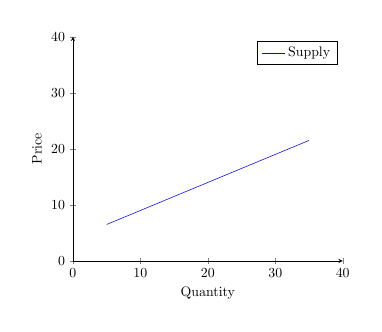
\begin{tikzpicture}[scale = 0.5]
                  \begin{axis}[
                          axis lines = left,
                          xlabel = Quantity,
                          ylabel = Price,
                          ymax = 40,
                          xmax = 40,
                          ymin = 0,
                          xmin = 0,
                          legend entries = {Supply}
                      ]
                      \addplot [
                          domain=5:35,
                          samples=10,
                          color=blue,
                      ]
                      {0.5*x + 4};
                  \end{axis}
              \end{tikzpicture}
              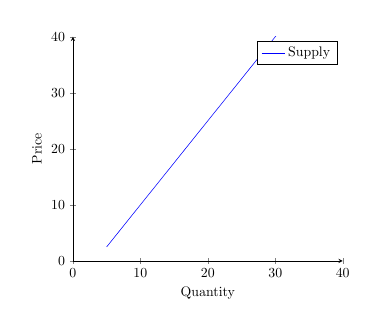
\begin{tikzpicture}[scale = 0.5]
                  \begin{axis}[
                          axis lines = left,
                          xlabel = Quantity,
                          ylabel = Price,
                          ymax = 40,
                          xmax = 40,
                          ymin = 0,
                          xmin = 0,
                          legend entries = {Supply}
                      ]
                      \addplot [
                          domain=5:35,
                          samples=10,
                          color=blue,
                      ]
                      {1.5*x - 5};
                  \end{axis}
              \end{tikzpicture}
          \end{center}
          The factors that affect supply elasticity are the following:
          \begin{itemize}
            \item Storage ease
            \item Additional input availability
            \item The capacity to produce more
            \item Ease of market entry/exit
            \item Response time availability
          \end{itemize}
\end{itemize}
Some other, less important elasticities are:
\begin{itemize}
    \item Labor supply elasticity
    \item Advertising Elasticity (and cross-advertising elasticity)
    \item Crime elasticity
\end{itemize}
\section{Intervening in Markets}
The government can influence the market through actions like taxes, regulations, subsidies, among others.\\
This does not, however, stop market forces, it just changes how much things benefit each of the parties in transactions.\\
Some taxes are:
\begin{itemize}
    \item Excise tax: tax on each unit sold, collected from supplier $\leftarrow$ focus of the class
    \item Ad Valorem tax: percentage tax
\end{itemize}
A tax on sellers is seen as a rise in marginal cost of production. It causes a parallel shift of the supply curve:
\begin{center}
    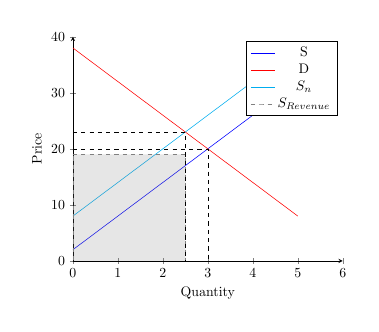
\begin{tikzpicture}[scale = 0.5]
        \begin{axis}[
                axis lines = left,
                xlabel = Quantity,
                ylabel = Price,
                ymax = 40,
                xmax = 6,
                ymin = 0,
                xmin = 0,
                legend entries = {S, D, $S_n$, $S_{Revenue}$}
            ]
            \addplot [
                domain=0:5,
                samples=10,
                color=blue,
            ]
            {6*x + 2};
            \addplot [
                domain=0:5,
                samples=10,
                color=red,
            ]
            {-6*x + 38};
            \addplot [
                domain=0:4,
                samples=10,
                color=cyan,
            ]
            {6*x + 8};
            \addplot [gray, dashed, fill = gray, fill opacity = 0.2] coordinates {(0,19) (2.5,19) (2.5, 0)} \closedcycle;
            \addplot [black, dashed] coordinates {(0,20) (3,20) (3,0)};
            \addplot [black, dashed] coordinates {(0,23) (2.5,23) (2.5,0)};
        \end{axis}
    \end{tikzpicture}
\end{center}
It causes an increase in price and a reduction in quantity. It also reduces the amount that the seller keeps.\\
If the tax were instead on the buyer, the marginal benefit of the buyer reduces:
\begin{center}
    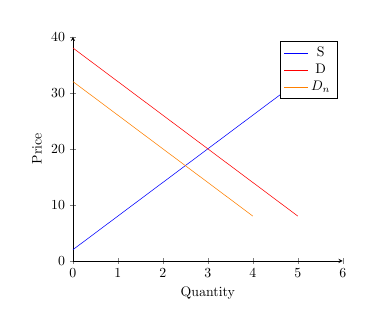
\begin{tikzpicture}[scale = 0.5]
        \begin{axis}[
                axis lines = left,
                xlabel = Quantity,
                ylabel = Price,
                ymax = 40,
                xmax = 6,
                ymin = 0,
                xmin = 0,
                legend entries = {S,D,$D_n$}
            ]
            \addplot [
                domain=0:5,
                samples=10,
                color=blue,
            ]
            {6*x + 2};
            \addplot [
                domain=0:5,
                samples=10,
                color=red,
            ]
            {-6*x + 38};
            \addplot [
                domain=0:4,
                samples=10,
                color=orange,
            ]
            {-6*x + 32};
        \end{axis}
    \end{tikzpicture}
\end{center}
The posted price is what goes to the seller, and $paid - posted = tax$, which is what goes to the government.\\
To solve these systems, we need to get both price equations, and then add the tax to the price for whichever entity is receiving the tax.\\
\defn{Tax Wedge}{(Tax)$\times$(New Quantity in Market)}
\begin{center}
    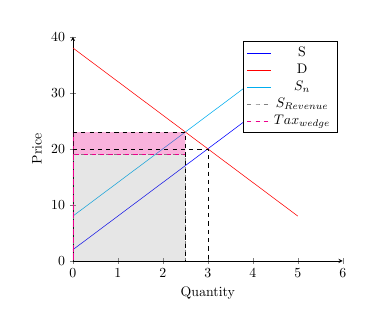
\begin{tikzpicture}[scale = 0.5]
        \begin{axis}[
                axis lines = left,
                xlabel = Quantity,
                ylabel = Price,
                ymax = 40,
                xmax = 6,
                ymin = 0,
                xmin = 0,
                legend entries = {S, D, $S_n$, $S_{Revenue}$, $Tax_{wedge}$}
            ]
            \addplot [
                domain=0:5,
                samples=10,
                color=blue,
            ]
            {6*x + 2};
            \addplot [
                domain=0:5,
                samples=10,
                color=red,
            ]
            {-6*x + 38};
            \addplot [
                domain=0:4,
                samples=10,
                color=cyan,
            ]
            {6*x + 8};
            \addplot [gray, dashed, fill = gray, fill opacity = 0.2] coordinates {(0,19) (2.5,19) (2.5, 0)} \closedcycle;
            \addplot [magenta, dashed, fill = magenta, fill opacity = 0.3] coordinates {(0,23) (2.5,23) (2.5, 19) (0,19)} \closedcycle;
            \addplot [black, dashed] coordinates {(0,20) (3,20) (3,0)};
            \addplot [black, dashed] coordinates {(0,23) (2.5,23) (2.5,0)};
        \end{axis}
    \end{tikzpicture}
\end{center}
\defn{Statutory Burden}{Burden of needing to pay taxes}\\
\defn{Economic Burden}{Burden created by after-tax prices}\\
\defn{Tax incidence}{Division of Economic Burden}\\
Tex incidence is independent of statutory burden. It can fall in some combination upon buyers and sellers. The policy alone is not enough to know the economic burden.\\
The market is what defines tax incidence, not the government.\\
\end{document}